% $ based on Id: sample_english-v1.2.tex,v 1.2 2007/04/12 21:05:22 zlb Exp $
% $Id: sample_english.tex 6 2011-01-24 13:13:33Z hsqi $

\documentclass[english]{cccconf}
%\documentclass[usemulticol,english]{cccconf}
\usepackage[comma,numbers,square,sort&compress]{natbib}
\usepackage{epstopdf}
\usepackage{comment}
\usepackage{subcaption}
\usepackage{color}
\usepackage{lipsum}
\usepackage{multicol}
\usepackage{amssymb}
\usepackage{amsmath}
\usepackage{bm}
\usepackage{amsfonts}
\usepackage{multirow}
\usepackage{graphicx}
\usepackage{mathtools, amssymb}
\usepackage[comma,numbers,square,sort&compress]{natbib}
\usepackage{CJK}
\usepackage{graphicx}
\usepackage{epsfig}
\usepackage{float}
\usepackage{multirow}
\usepackage{algorithm}
\usepackage{algorithmic}
\usepackage{indentfirst}
\usepackage{booktabs}
\usepackage{amsmath}



\begin{document}

\title{Competition of Social Opinions on Two Layer Networks}

% Note: the first argument in the \affiliation command is optional.
% It defines a label for the affiliation which can be used in the \aref
% command. If there is only one affiliation for all authors, then the
% optional argument in the \affiliation command should be suppressed,
% and the \aref command should also be removed after each author in
% \author command, in this case the affiliation will not be numbered.
% \author{First Author, Second Author, Third Author}
% \affiliation{Chinese Academy of Sciences, Beijing 100190, P.~R.~China\email{ccc@amss.ac.cn}}

\author{Cho Hyunchel \aref{amss,hit},
        A. Mahmood \aref{amss,hit},
        Lin Wang \aref{amss,hit}}
\affiliation[amss]{Department of Automation, Shanghai Jiao Tong University, Shanghai 200240, P.~R.~China}
\affiliation[hit]{Key Laboratory of System Control and Information Processing, Ministry of Education of China, Shanghai 200240, P.~R.~China
        \email{leighsix@naver.com}\email{arfan499@sjtu.edu.cn}\email{wanglin@sjtu.edu.cn}}

\maketitle

\begin{abstract}
Social conflict can be explained with competition network of two layers. This paper is investigated for a model with the competition between two-layer opinions, where the first layer is opinion formation and the second layer is decision making, on interconnected networks. Networks show the two interacting social sectors, the civilians, and representatives. Layer A is civilian opinion layer consists of four states $(-2, -1, +1, +2)$. These states describe the level of influence of opinion dynamics with reinforcement parameter $\gamma$. The layer B is the decision making layer that consists of only two states $(+1, -1)$.  This layer can influence the decision dynamics with the probability in which decision is proportional to the number of interaction with the opposite opinion population raised to the power of $\beta$. Starting with a polarized competition case, layer A is all positive and layer B is all negative. In this paper, we create new models by changing the network structure, and compare these models with the pre-existing model. Then conditions are investigated that have the influence to opposite side and that make consensus in the interconnected network. This study could help to analyze social networks, such as legalization of social issues and prediction of vote results. Further more, it could contribute to solving the social conflict.
\end{abstract}

\keywords{Complex Network, Interconnected Networks, Opinion Dynamics, Decision Making System, Consensus}

% Please remove or comment out the following line if the footnote is not necessary
\footnotetext{This work was supported by the National Natural Science Foundation of China under Grant Nos 61873167, 61473189, 61773255, the Natural Science Foundation of Shanghai (No. 17ZR1445200), and the Science Fund for Creative Research Groups of the National Natural Science Foundation of China (No. 61521063).}

\section{Introduction}
 People have their own opinions, and sometimes they change their opinions in response to others that hold views on given issues. Their opinions are reflected to the leader to make laws and vital decision for their countries. Also, the leaders or representatives affect the individuals that belong to their groups. In this case, the social phenomenon can be explained by dividing two layers, social opinion layer and decision making layer. It has to be considered as interconnected networks, where nodes belong to different layers interact with each other\cite{newman2010,boccaletti2014,domenico2013,tomasini2015,namkhanhvu2017}. In various situations ranging from voting to adoption of new policies, it is widely recognized that opinion formation and decision making formation have mutual interaction as interconnected network\cite{mikko2013, danziger2019}. And sometimes, opinion formation could be opposed to decision making formation. These situations often make social conflict and cause social confusion. To figure out these social conflicts, it is needed to understand and analyze the competition of interconnected networks. So far, physics and computer science have researched these social conflict by modeling and analyzing the complex systems\cite{huberman2004, zuev2012, laguna2004, masuda2015}. The researches include opinion dynamics, voter model, game theory and many more\cite{bianconi2018}. 
 
 In this paper, opinion dynamics are discussed by analyzing the dynamics of a competing two-layer social network, based on the pre-existed research\cite{alvarez2016, gomez2015, diep2017, rocca2014}. The model consists of interconnected two layer networks. One layer has the function of social opinion and its own dynamics. The dynamics of the social opinion layer is a kind of opinion dynamics which are also known as M-model\cite{rocca2014}, that includes compromise function and persuasion function. The other layer also has the function of decision-making and its own dynamics. The dynamics of the decision making layer is the language competition dynamics that are also called as Abrams-Strogatz model\cite{abrams2003, vazquez2010}. And, the initial condition of the two layers is assumed to be in opposite states, social opinion layer has all positive states, decision making layer has all negative states.
 
As the result of pre-existed research, interconnected competition of the social network have been researched by finding the threshold or critical point for consensus\cite{alvarez2016, gomez2015, diep2017}. It has been proved that the system can make positive consensus, negative consensus or coexistence parts in interconnected competition of the social network\cite{alvarez2016}. And it is shown that the number of external degree is very important to change the state of layers\cite{gomez2015}. We develop the previous modeling and research to find out the characteristics of interconnected networks. By switching the network structure of each layer, such as changing the number of nodes or the number of edges, we can see how the consensus or coexistence states change and what conditions make the social consensus. This can help to explain social networks phenomena, such as social conflict between social opinion and the congress. Therefore, this research could be used as a tool for analyzing legislation problems, making efficient decision-making system and solving the social conflict. 

The paper is organized as follows. In section 2, the Basic Model is introduced and the dynamics, that is applied to each layer, are described.  In section 3, the simulation results for the basic model and revised models are presented. In section 4 the characteristics of each model are described through the comparison and analysis. Finally, in section 5, the simulation results will be summarized and our findings are concluded.

\section{Modeling}
The Basic Model of this interconnected network consists of two layers that are called as layer A and layer B, individually. Each layer consists of random regular network that has $N$ nodes with $k$ internal edges on the same layer. Each node of a layer is connected with a random node on the other layer. That means all the node has only 1 external un-directed edge.

Dynamics of layer A follows opinion dynamics, called as $M$-model. This dynamics is applied to layer A nodes and layer B nodes that are connected with layer A nodes. Each layer A node updates its state step by step. But, layer B nodes do not change their states, because layer B nodes is applied to decision making dynamics. The state of each node is represented by integer number $j$ and $k$. And the maximum state of nodes is $M$. If $k$ and $j$ are connected on networks (it includes internal and external edges), the dynamics is like this formula\cite{gomez2015}. \\
i) Compromise : if they have opposite orientations, their states become more moderate with probability $q$ :
\begin{align*}
  \mbox{if } j<0 \mbox{ and } k>0  \Rightarrow (j, k) \rightarrow (j^r, k^l) \mbox{ with } prob.q\\
  \mbox{if } j>0 \mbox{ and } k<0  \Rightarrow (j, k) \rightarrow (j^l, k^r) \mbox{ with } prob.q
\end{align*}
If $j = \pm1$ and $k = \mp1$, one switches orientation at random:
\begin{align*}
(\pm 1, \mp 1)\rightarrow \left\{\begin{matrix}
(+1, +1) \quad with \quad prob.q/2
\\(-1, -1)\quad with \quad prob.q/2
\end{matrix}\right.
\end{align*}
ii) Persuasion : if they have the same orientation, their states become more extreme with probability $p$ :
\begin{align*}
  \mbox{if } j<0 \mbox{ and } k<0  \Rightarrow (j, k) \rightarrow (j^l, k^l) \mbox{ with } prob.p\\
  \mbox{if } j>0 \mbox{ and } k>0  \Rightarrow (j, k) \rightarrow (j^r, k^r) \mbox{ with } prob.p
\end{align*}
Here, $k^r$ and $k^l$ denote the right and left neighboring states of $k$, defined as
\begin{align*}
k^r &= \left\{\begin{matrix}
1,\quad for\quad k= -1
\\ M,\quad for \quad k=M
\\ k+1,\quad otherwise
\end{matrix}\right. &
k^l &= \left\{\begin{matrix}
1,\quad for\quad k= -1
\\ M,\quad for \quad k=M
\\ k+1,\quad otherwise
\end{matrix}\right.
\end{align*}
As the initial condition for Basic Model, the dynamics on layer A has M-model dynamics with $M = 2$. If $M = 2$, the opinion state of each node can have four possible values such as $S^A$ = $-2$, $-1$, $+1$, and $+2$, where the sign of $S^A$ represents its opinion orientation and its absolute value $|S^A|$ measures the intensity of its opinion. So, $|S^A|=2$ represents to a positive or a negative extremist, while  $|S^A|=1$ correspond to a moderate opinion of each side. But, as the initial condition, nodes of layer A have only positive values, half nodes of the layer are $+1$ and the others are $+2$. In case of interaction between layer A node and layer B node, layer A node follows opinion dynamics formula, but the state of layer B node does not change. In other words, the state of layer B affects layer A, but this dynamics does not affect state of layer B node. For example, one of layer A node, $S_i = +2$ is connected with one of layer B node, $S_j = -1$. In this case, $S_i$ will change into $S_i = +1$ with $prob.q$. But $S_j$ will not change. That means layer B node states have influence on layer A nodes.

The dynamics of layer B follow language competition dynamics as the decision-making dynamics\cite{abrams2003, vazquez2010}. Language competition dynamics follow the formula below. The state of node i in layer B changes with this probability.
\begin{equation}
P_B(S_i \rightarrow -S_i)= \left \{\frac{n^{-S_i}}{i_i + e_i}\right \}^\beta
\end{equation}
$i_i$ is the number of internal edges and $e_i$ is the number of external edges. $n^{-S_i}$ is the number of neighbors of i with opposite state $-S_i$. $\beta(\geq 0)$ is the volatility exponent that measures how prone a node change state. This formula means that the more the nodes are connected with the opposite state, the easier the nodes can be changed into the opposite state.
The states of layer B nodes can be $+1$ and $-1$. But, as an initial condition, the states are only $-1$. By this formula, the state of layer A has influence on change of layer B node states.

In summary, states of layer A nodes are positive states of $+1$ and $+2$ as an initial condition, and the states of layer B node, which is connected with layer A, affects the state change of the node on layer A. Inversely, states of layer B nodes are negative states of $-1$ as an initial condition, and the states of nodes, which is connected with a node of layer B, have influence on the change of layer B nodes. Under these conditions, it would be found out how consensus happen and what conditions make consensus happen.\\
\begin{figure}[!htb]
  \centering
  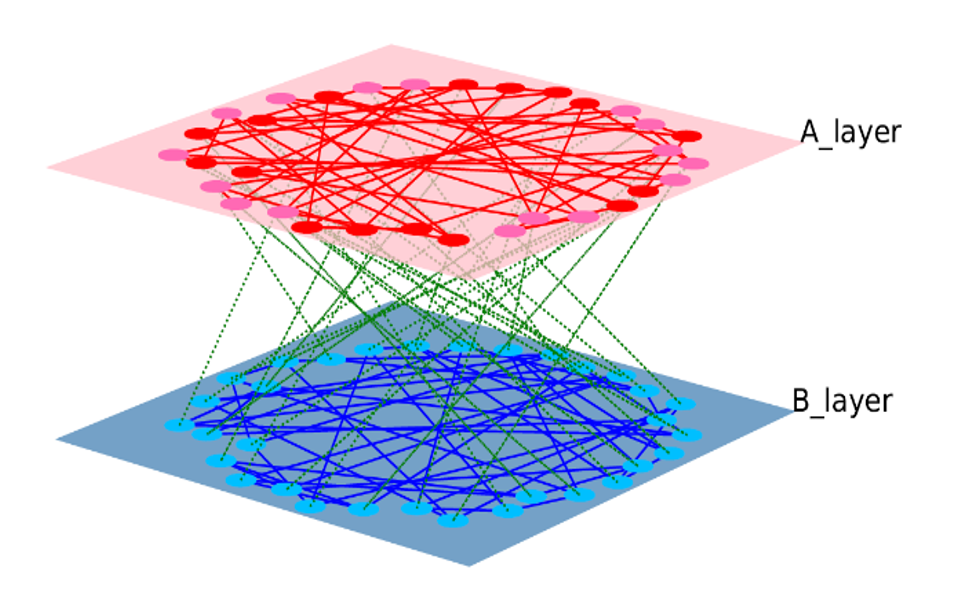
\includegraphics[width=\hsize]{FIG1.png}
  \caption{Competition of Interconnected Network}
  \label{Fig1}
\end{figure}
\begin{figure*}[!htb]
  \centering
  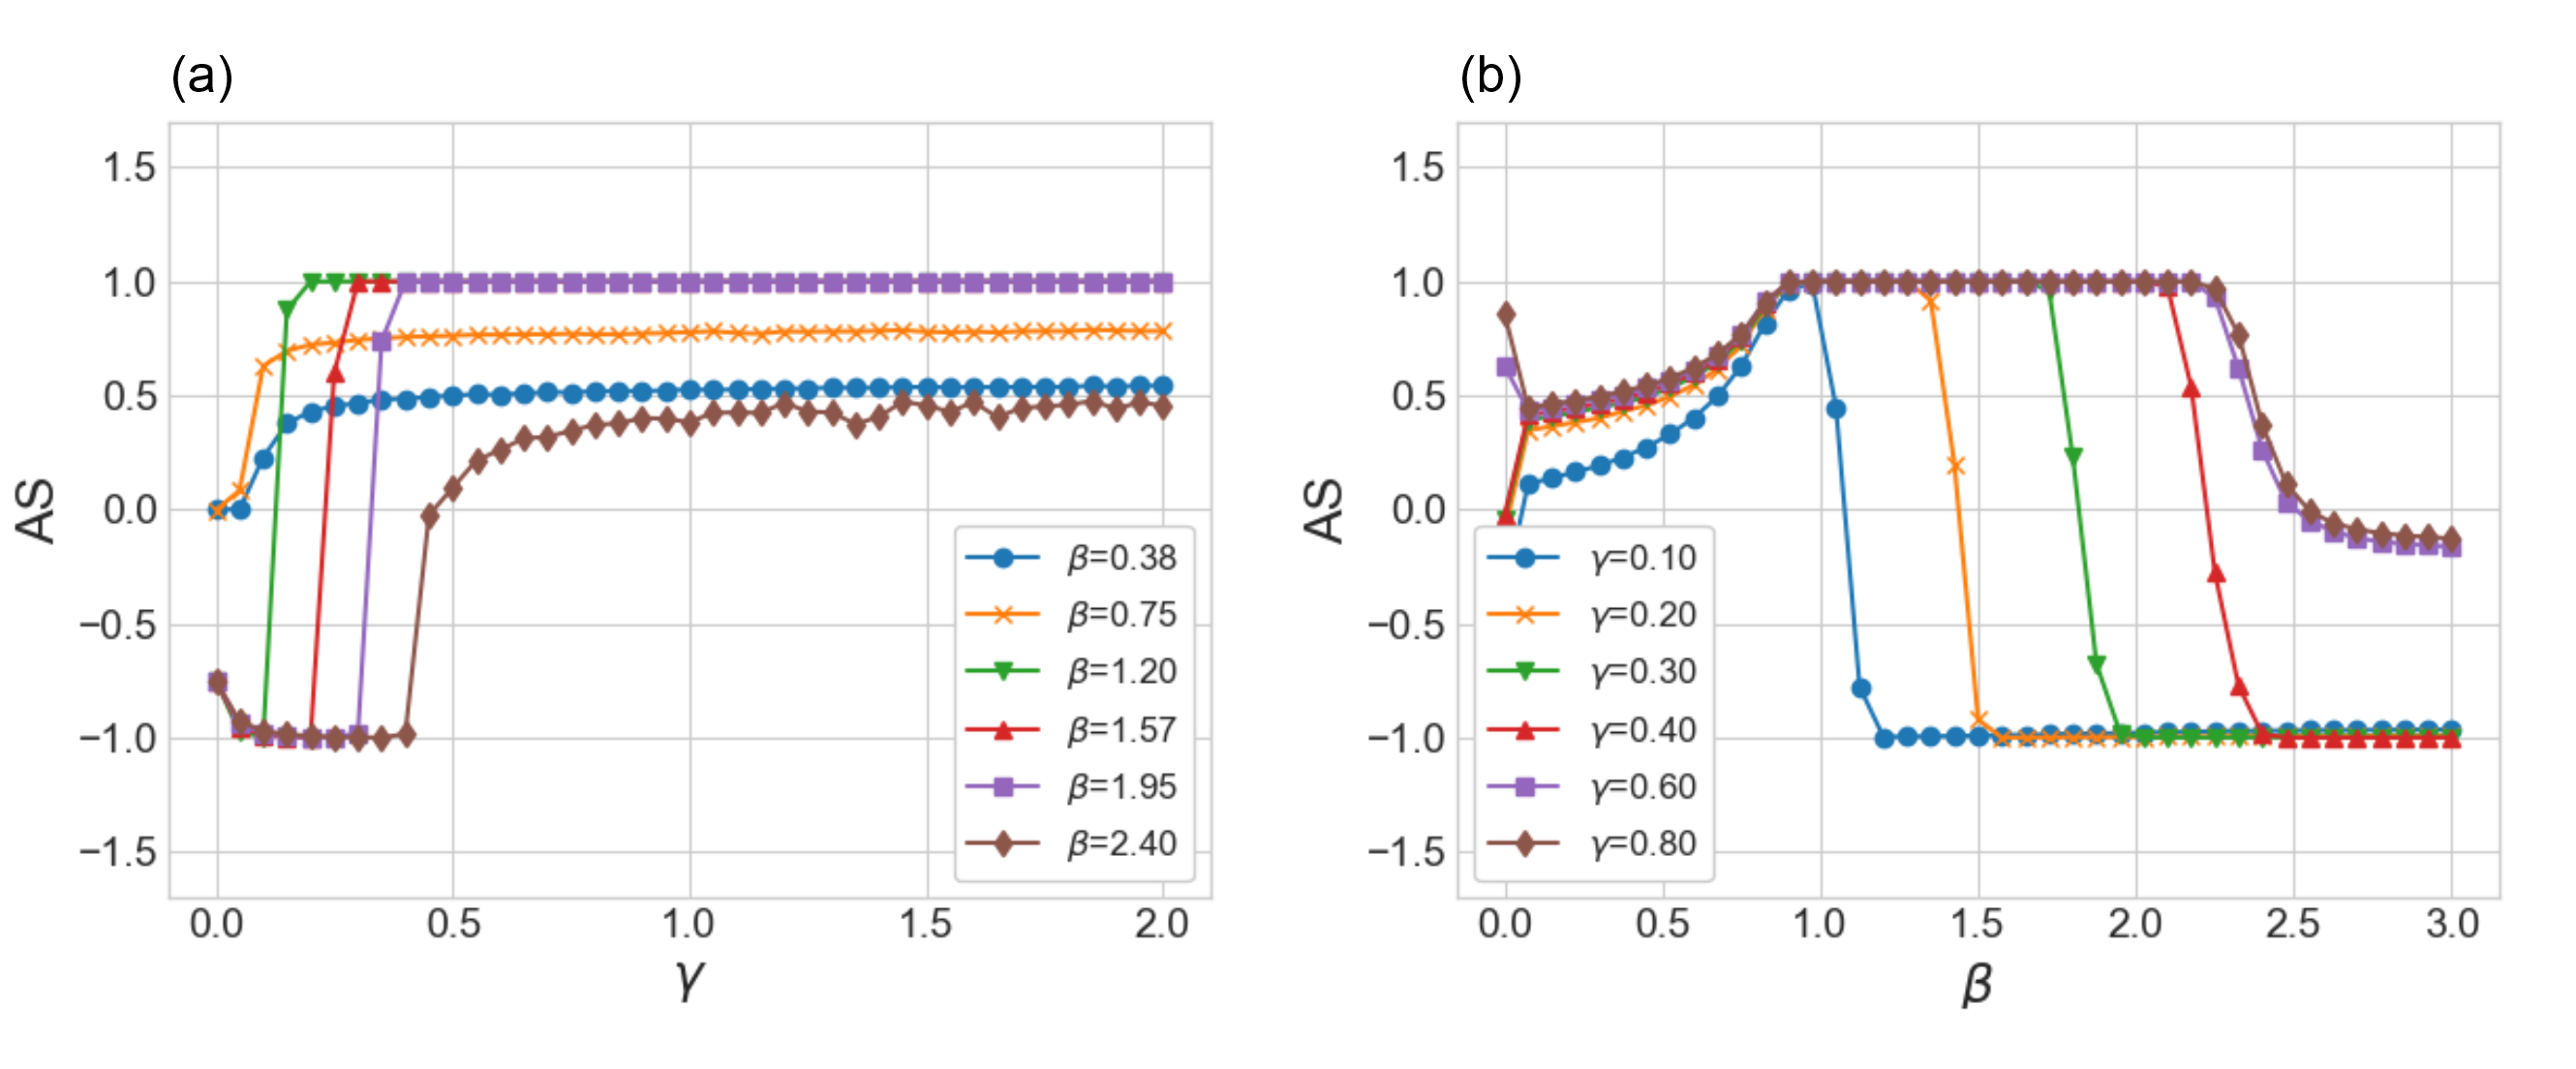
\includegraphics[width=\hsize]{FIG2.png}
  \caption{(a) $\beta$-Average State chart according to some $\beta$ values. (b) $\gamma$-Average State chart according to some $\gamma$ values.}
  \label{Fig2}
\end{figure*}
\section{Simulation Result}
We organized interconnection networks in Section 2. Each layer consists of a random regular network with each node having the same degrees\cite{bela2001}. Each node consists of five internal edges and one external edge. Layer A dynamics has the probability $p$ and probability $q$ denoted by $M$-model. We observe how the state changes by switching the probability $p$ and probability $q$. To simply represent the probability $p$ and probability $q$ together, we set the value $p+q=1$, and $\gamma = p/q$. $\gamma$ represents the tendency of opinion such as extreme or moderate\cite{alvarez2016}. For layer B dynamics, by switching $\beta$, the changes of states are investigated, where $\gamma$ scale is $0$ to $2$, and $\beta$ scale is $0$ to $3$, basically. But, $\beta$ scale depends on the total number of degrees. So, when the number of degrees is changed, the $\beta$ scale would be adjusted properly to Basic Model scale.

To implement the interconnected dynamics, one step consists of two layers dynamics, where layer A dynamics and layer B dynamics are carried out step by step. Basically, $30$ steps are taken. And these procedure is repeated by $100$ times to calculate the average states change of each layer. And we calculated \textit{`Average State'} that can measure two layer state. 
\begin{equation}
AS = avg\left( {\sum\limits_{{K^A}} {S_i^A/M} } \right) + avg\left( {\sum\limits_{{K^B}} {S_i^B} } \right)
\end{equation}
With \textit{`Average State'(AS)}, it could be checked whether the consensus happens or not in accordance with $\gamma$ and $\beta$ changing.  If the positive consensus happens, it would be close to the value of $+2$ and if the negative consensus happens, it would be close to the value of $-2$. The values between $+2$ and $-2$ are not on the consensus yet, so these states are considered as belonging to the coexistence part.
And, the Basic Model would be redesigned by changing the network structures. To compare revised models with Basic Model and estimate their structural properties, we use and compute $4$ kinds of measures for simulation results, including \textit{`AS'}, \textit{`Positive Consensus Ratio'(PCR)}, \textit{`Negative Consensus ratio'(NCR)}, \textit{`Consensus Ratio'(CR)}.

First, the Basic Model is simulated, and then other simulations would be implemented with revised network structures.

\subsection{Basic Model Result}
Basic model simulation results are shown in Fig.~\ref{Fig2} and Fig.~\ref{Fig3}. Fig.~\ref{Fig2}(a) shows that when $\gamma$ increases, if $\beta$ is in some range$(1.2 < \beta < 1.95)$, it normally tends to make positive consensus. But, if $\beta$ is too low or too large, it cannot make consensus.
In Fig.~\ref{Fig2}(b), as $\beta$ increases, it normally tends to make positive or negative consensus. But, when $\gamma$ is very low($\gamma \le 0.1$), it cannot make positive consensus. On the other hand, when $\gamma$ is large enough, it can make positive consensus. But, $\beta$ is large enough, it can change into negative consensus. When both of $\gamma$ and $\beta$ are large enough, its state is in the coexistence part. 

In Fig.~\ref{Fig3}, that shows the states of two layers according to $\gamma$ and $\beta$. The $X$-axis is the $\gamma$ and the $Y$-axis is the $\beta$, and the $Z$-axis represents the average summation of the nodes' states in layer A and B. With this simulation properties, the consensus and two layer states would be estimated as \textit{AS total}, \textit{CR}, \textit{PCR}, and \textit{NCR}. \textit{AS total} means the summation of \textit{AS} with changing $\gamma$ and $\beta$. \textit{CR} is the ratio of consensus part in the simulation result. \textit{PCR} is the ratio of positive consensus in the simulation result. And \textit{NCR} is the ratio of negative consensus part in the simulation result.  
\begin{figure}[!htb]
  \centering
  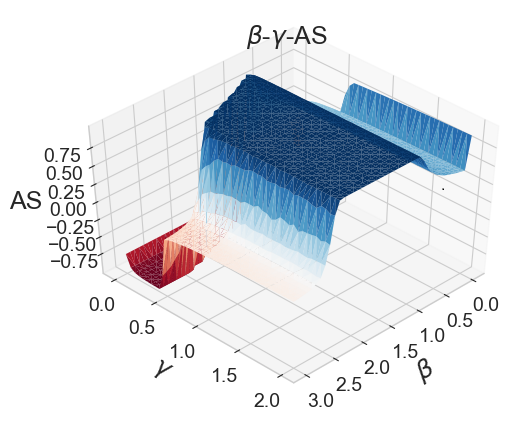
\includegraphics[width=\hsize]{FIG3.png}
  \caption{Basic model result : Average state of layer A and B with changing $\gamma$ and $\beta$}
  \label{Fig3}
\end{figure}
In Fig.~\ref{Fig3}, the closer the color is to be blue, the more it has positive consensus. And the closer the color is to be red, the more it has negative consensus. A light and white areas have coexistence with positive states and negative states mixed. This chart has two areas for coexistence, when $\beta$ is very low or high. Which means, when $\beta$ is in some range, interconnected network can make positive or negative consensus with $\gamma$ value.
\begin{figure*}[!htb]
  \centering
  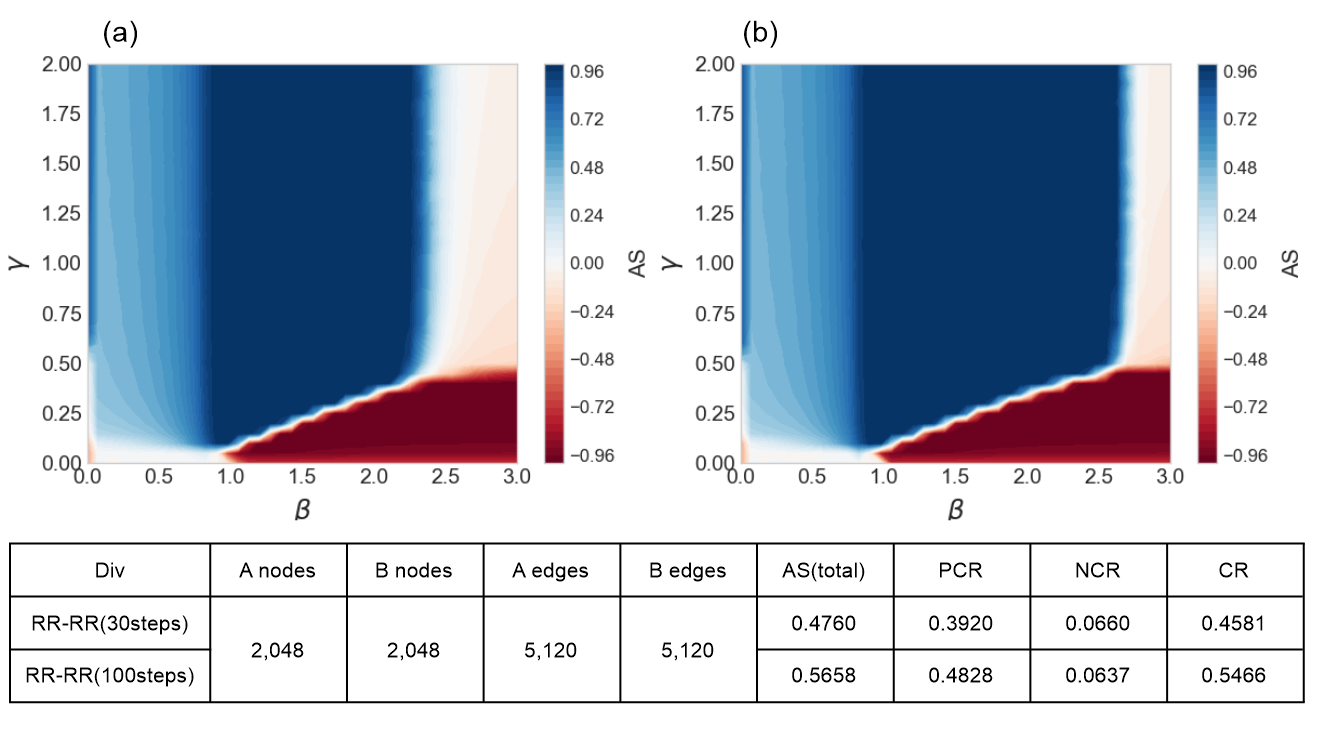
\includegraphics[width=\hsize]{FIG4.png}
  \caption{Comparison between 30 steps dynamics result and 100 steps dynamics result}
  \label{Fig4}
\end{figure*}
With Basic Model simulation, the dynamics steps are increased from $30$ steps to $100$ steps. Fig.~\ref{Fig4} provides the comparison between $30$ steps and $100$ steps dynamics. In Fig.4 table, \textit{CR} and \textit{PCR} of 100 steps dynamics  has larger than $30$ steps dynamics. As the dynamics steps are increased, the layer states are more stable and positive consensus happens increasingly. 

\subsection{Leader Model Result}
\begin{figure}[!htb]
  \centering
  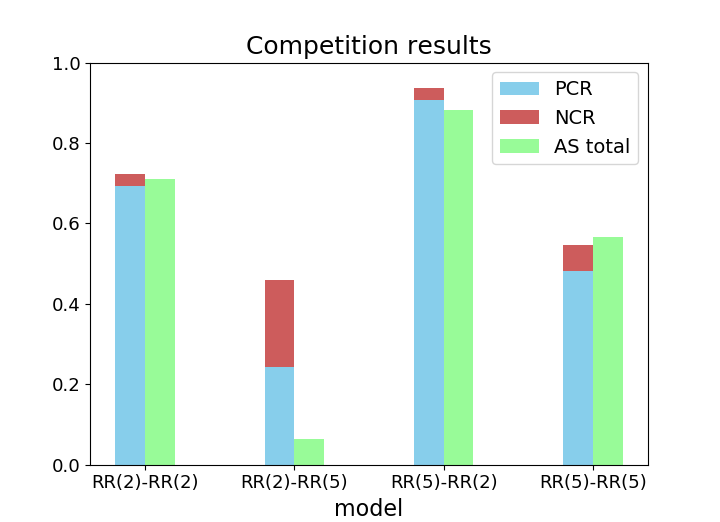
\includegraphics[width=\hsize]{FIG5.png}
  \caption{Leader Model results(BM : Basic Model, LM(n) : Leader Model where the number of layer B nodes are reduced by 1/n)}
  \label{Fig5}
\end{figure}
The Leader Model is the revised model where the number of layer B nodes is reduced at certain rate such as $1/16$ or $1/4$, and increase the number of external edges by certain rate like $16$ times or $4$ times. In other words, each layer A node has one external edge, but each layer B node has $16$ or $4$ external edges. That is, as social network relation, it can be analyzed that one node of layer B represents the nodes of layer A. $\gamma$ scale is same as the Basic Model. But, $\beta$ scale depends on the number of degrees. So the $\beta$ scale is adjusted to same values as the Basic Model. Leader Model simulations are implemented with $6$ kinds of rates$(1/64, 1/32, 1/16, 1/8, 1/4, 1/2)$. Fig.~\ref{Fig5} shows the Leader Model simulation results. Comparing \textit{LMs} with Basic Model, \textit{CR} and \textit{PCR} are all increased remarkably. Leader Models have more positive consensus part than Basic Model. It shows that as the number of B nodes(Leader) are decreased, it is easy to make positive consensus. Comparing \textit{LM(8)} with other \textit{LMs}, \textit{LM(8)} has most positive consensus part. As the number of layer B nodes is less than \textit{LM(8)},  \textit{CR} and \textit{PCR} are decreased and \textit{NCR} is increased slightly. Also, as the number of layer B nodes is more than \textit{LM(8)}, \textit{CR} and \textit{PCR} are decreased. Among \textit{LMs}, it is found out that there is the efficient number of B nodes(Leader) for making positive consensus.   

\subsection{Different Structural Networks Model Result}
So far, each layer of the interconnected network consisted of random regular network that has the same number of edges for each node. Now, the simulation would be implemented with changing network structures or the number of internal edges. 
\subsubsection{Changing Network Structure}
\begin{figure}[!htb]
  \centering
  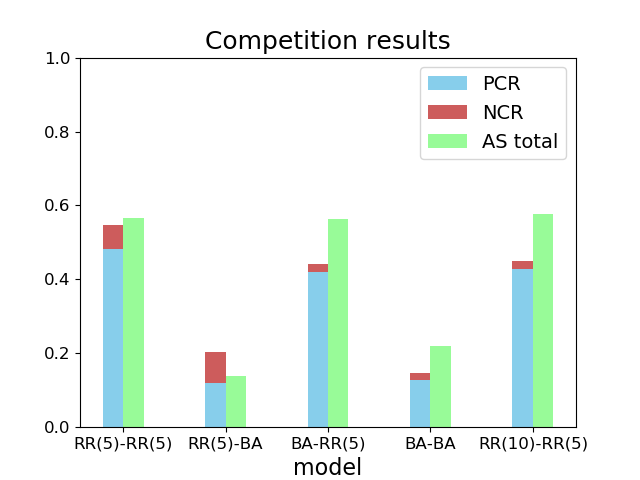
\includegraphics[width=\hsize]{FIG6.png}
  \caption{Comparison of models with different network structure}
  \label{Fig6}
\end{figure}
To estimate interconnected network with different network structure, \textit{Barabasi-Albert network(BA)} structure was applied for layer A\cite{barabasi1999, kimsangwoo2012}. To evaluate the influence of network structure, 5 simulations were implemented with changing network structures. The BA network were applied to both layers or switched on each layer. And, Because layer A of \textit{BA} network has total $10,215$ edges, random regular network(\textit{`RR(10)-RR(5)'} under the similar conditions such as the number of nodes and edges was also simulated.  \textit{RR(10)-RR(5)} means that layer A has random regular(\textit{RR}) network with $10$ internal edges per each node and layer B has random regular(\textit{RR}) network with $5$ internal edges per each node.  The simulation results are shown as Fig.~\ref{Fig6}. The result properties of \textit{BA-RR} and \textit{RR(10)-RR(5)} are almost same. The gap of \textit{CR} is less than 0.007. The structure of network make no difference of consensus results. In case of \textit{BA-BA}, the \textit{CR} is the least ratio for consensus. \textit{`BA-BA'} structure has too many internal edges. Therefore, it is analyzed that it is hard to make consensus due to inner conflict on each layer. 
\subsubsection{Changing the number of internal edges}
Next, the model were redesigned by changing the number of internal edges. The number of internal edges on each node is changed to $2$ or $5$.
\begin{figure}[!htb]
  \centering
  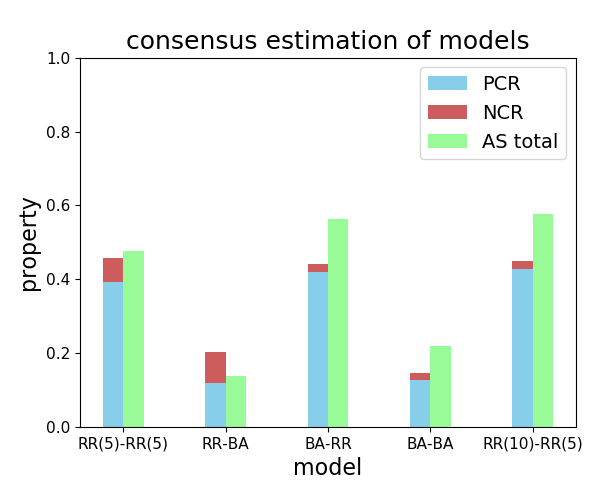
\includegraphics[width=\hsize]{FIG7.png}
  \caption{Comparison according to changing the number of internal edges on layer A and B}
  \label{Fig7}
\end{figure}
Fig.~\ref{Fig7} shows the simulation result with changing the number of internal edges. \textit{RR(5)-RR(2)} has the most \textit{PCR}. \textit{RR(2)-RR(5)} has the most \textit{NCR}. The number of edges on layer A has the tendency to keep positive state. The number of edges on layer B has the tendency to keep negative state. The number of internal edges have the influence on consensus result.

\section{Comparison and Analysis}
\begin{table*}[!htb]
	\centering
	\caption{Consensus properties of Simulation Models}
	\label{tab1}
	\begin{center}
		\begin{tabular}{c|c|c|c|c|c|c|c|c} \hline\hline
			Div               & A nodes & B nodes & A edges & B edges & AS(total) & PCR    & NCR    & CR       \\ \hline \hline
			Basic Model(30)   & 2,048   & 2,048   & 5,120   & 5,120   & 0.9520    & 0.3968 & 0.0773 & 0.4741   \\ \hline
			Basic Model(100)  & 2,048   & 2,048   & 5,120   & 5,120   & 1.1315    & 0.4928 & 0.0759 & 0.5687   \\ \hline
			DSN Model(RR-BA)  & 2,048 	& 2,048   & 5,120   & 10,215  & 0.2794    & 0.1356 & 0.0993 & 0.2350   \\ \hline 
			DSN Model(BA-RR)  & 2,048 	& 2,048   & 10,215  & 5,120   & 1.1245    & 0.4236 & 0.0291 & 0.4527   \\ \hline
			DSN Model(BA-BA)  & 2,048 	& 2,048   & 10,215  & 10,215  & 0.4394    & 0.1446 & 0.0315 & 0.1761   \\ \hline
			RR(10)-RR(5)      & 2,048 	& 2,048   & 10,240  & 5,120   & 1.1551    & 0.4307 & 0.0286 & 0.4593   \\ \hline
			RR(2)-RR(2)       & 2,048 	& 2,048   & 2,048   & 2,048   & 1.4229    & 0.6930 & 0.0309 & 0.7240   \\ \hline 
			RR(2)-RR(5)       & 2,048 	& 2,048   & 2,048   & 5,120   & 0.1286    & 0.2427 & 0.2165 & 0.4593   \\ \hline 
			RR(5)-RR(2)       & 2,048 	& 2,048   & 5,120   & 2,048   & 1.7622    & 0.9066 & 0.0315 & 0.9381   \\ \hline
			Leader Model(2)   & 2,048 	& 1,024   & 5,120   & 2,560   & 1.2658    & 0.5863 & 0.0750 & 0.6613   \\ \hline    
			Leader Model(4)   & 2,048 	&  512    & 5,120   & 1,280   & 1.3902    & 0.6819 & 0.0781 & 0.7600   \\ \hline
			Leader Model(8)   & 2,048 	&  256    & 5,120   & 640     & 1.3535    & 0.6919 & 0.0856 & 0.7775   \\ \hline
			Leader Model(16)  & 2,048 	&  128    & 5,120   & 320     & 1.2701    & 0.6731 & 0.0988 & 0.7719   \\ \hline
			Leader Model(32)  & 2,048 	&   64    & 5,120   & 160     & 1.1508    & 0.6231 & 0.1125 & 0.7356   \\ \hline
			Leader Model(64)  & 2,048 	&   32    & 5,120   & 80      & 1.0128    & 0.5713 & 0.1219 & 0.6931   \\ \hline  \hline
		\end{tabular}
	\end{center}
\end{table*}

In this section, the simulation results are compared and analyzed to provide what conditions make the consensus on the interconnected networks. Based on Basic Model, two models were provided and $15$ simulations were implemented. Table.~\ref{tab1} shows simulation results of all models. Consensus and network state of each model are estimated with these simulation properties. Through comparison and analysis of these properties, three main results are derived. 
First, when dynamics steps are increased with Basic Model, \textit{PCR} and \textit{CR} are increased. It is analyzed that social opinion is likely to achieve the consensus if it was given enough time with stable reinforcement($\gamma$) above critical point.

Next, with Leader Model, 6 simulations were researched by changing the number of B nodes. As a result, all the Leader Model has more consensus ratio than the Basic Model. Among \textit{LMs}, \textit{LM(8)} has the most positive consensus part. When the number of layer B nodes is more or less than \textit{LM(8)}, \textit{CR} and \textit{PCR} are decreased. That means there is the efficient number of layer B nodes(leader) for making positive consensus.  

Last, the Basic Model is compared with Different Structural Networks Models. When the structure of layer A is changed to \textit{BA} network, there was no difference on consensus results. When the number of internal edges are changed on two layers, the simulation result shows the number of internal edges affects interconnected dynamics. One layer with more internal edges has the tendency to maintain its own state.

Through these three comparisons and analysis, we can provide three conditions that increase the likelihood of consensus with social opinion. Firstly, when the interconnected dynamics steps are increased with the reinforcement above critical point, there is a high possibility of consensus with social opinion. Secondly, Leader Model shows, if reducing the nodes of decision-making layer at certain rate and increasing the external edges, that can increase the probability of social opinion consensus. Thirdly, Different Structural Networks Model shows, social opinion layer requires more internal edges than opposite layer in order to make positive consensus. Because increasing the internal edges of social opinion has more tendency to keep social opinion states. 

\section{Conclusion}
In this work, we have researched competing interconnected network dynamics. Layer A is a layer of social opinion and has positive states as an initial condition. It is influenced by opinion dynamics. Layer B is a network representing decision making system and has a negative state as an initial condition. It is influenced by the language competition dynamics. When these two layers were connected and interacted, it showed how their states were changed with switching $\gamma$ and $\beta$. In the Basic Model, the simulation result shows three sections which are the negative consensus, the positive consensus, and the coexistence according to $\gamma$ and $\beta$. Based on this Basic Model, we have presented and simulated Leader Model, and Different Structural Networks Models. And 15 interconnected networks were simulated.

As a result, three conditions can increase the likelihood of consensus with social opinion layer. The first is to take enough time and keep social opinion with stable and enough $\gamma$. The second is to reduce nodes in the decision-making layer at certain rate and increase the external edges like the Leader Model. The third is to increase the internal edges of social opinion, because internal edges have an influence to strengthen and maintain states of the layer. More research will be needed to make generalized model and to be applied to real social networks. We think this research can contribute to providing the analysis tool of competing social networks such as the legalization or social decision-making system. Also, it could help to solve the social conflict by making consensus of two layer. As the future work, it would be very interesting to make the generalized model for competing interconnected network and find the key nodes and edges of interconnected network.

\begin{thebibliography}{0}
\bibitem{newman2010}
M. E. J. Newman, \textit{Networks: An Introduction}, Oxford University Press, 2010.

\bibitem{boccaletti2014}
S. Boccaletti et al, \textit{The structure and dynamics of multilayer networks}, Physics Reports 544, 2014.

\bibitem{domenico2013}
M. De Domenico et al, \textit{Mathematical Formulation of Multilayer Networks}, Physical Review X 3, 041022, 2013.

\bibitem{tomasini2015}
Marcello Tomasini, \textit{An Introduction to Multilayer Networks}, 10.13140/RG.2.2.16830.18243, 2015.

\bibitem{namkhanhvu2017}
Nam Khanh Vu, \textit{Robustness of Interconnected Complex Networks with Directed Dependency}, Yonsei University Department of Computer Science, 2017.

\bibitem{mikko2013}
Mikko Kivela et al, \textit{Multilayer Networks}, J. Complex Networks Volume 2. DOI : 10.1093/comnet/cnu016, 2013.

\bibitem{danziger2019}
Danziger, Michael M. et al, \textit{Dynamic interdependence and competition in multilayer networks}, Nature Physics Volume 15. pp.178-185, 2019.

\bibitem{huberman2004}
Wu F. and Huberman B.A, \textit{Social structure and opinion formation}, arXiv.org:cond-mat/0407252v3, 2004

\bibitem{laguna2004}
M. F. Laguna et al, \textit{The dynamics of opinion in hierarchical organizations}, arXiv.org:nlin/0404024, 2004 

\bibitem{masuda2015}
Naoki Masuda, \textit{Opinion control in complex networks}, New Journal of Physics, Volume 17, 2015.

\bibitem{zuev2012}
Zuev A S and Fedyanin, 
\textit{Models of opinion control for agents in social networks}, Automation and Remote Control Volume 73 Issue 10, pp.1753–1764, 2012 

\bibitem{bianconi2018}
G. Bianconi, \textit{Multilayer Networks: Structure and Function}, Oxford University Press, 2018.

\bibitem{alvarez2016}
Alvarez Zuzek et al, \textit{Interacting Social Processes on Interconnected Network}, PLoS ONE. 11. 10.1371/journal.pone.0163593, 2016.

\bibitem{gomez2015}
Gomez Gardenes J. et al, \textit{Layer-layer competition in multiplex complex network}, Phil. Trans. R. Soc. A 373:20150117, 2015

\bibitem{diep2017}
H.T. Diep et al, \textit{Dynamics of two-group conflicts: A statistical physics model}, Physica A: Statistical Mechanics and its Applications Volume 467. pp.183 - 199, 2017.

\bibitem{rocca2014}
C. E. La Rocca et al, \textit{The influence of persuasion in opinion formation and polarization}, Europhys. Lett. 106, 40004, pp.1-2, 2014.

\bibitem{abrams2003}
M Abrams et al, \textit{Modelling the dynamics of language death}, Nature.424.900. DOI : 10.1038/424900a, 2003.

\bibitem{vazquez2010}
 F. V{\'a}zquez et al, \textit{Agent based models of language competition: macroscopic descriptions and order–disorder transitions}, Journal of Statistical Mechanics: Theory and Experiment P04007, 2010.

\bibitem{bela2001}
 Bela Bollobas, \textit{Random Graphs}, 2nd edition, Cambridge University Press, section 2.4: Random Regular Graphs, 2001.

\bibitem{barabasi1999}
Barabasi A. L., Albert R, \textit{Emergence of Scaling in Random Networks}, Science 286, 509, DOI: 10.1126/science.286.5439.509, 1999.

\bibitem{kimsangwoo2012}
Kim Sangwoo, \textit{Structure and dynamics of complex networks}, Yonsei Univ, 2012.

\end{thebibliography}

\end{document}



































